% !TeX root = Protokoll.tex
%In diesem Versuch wird der Umgang mit modellierten Schwingungen veranschaulicht.
%Dazu werden sowohl Spannungen frequenz- als auch amplitudenmoduliert und demoduliert.
\subsection{Schwingung und Frequenzspektrum einer Amplitudenmodellierten Spannung}
\begin{figure}[h!]
	\centering
	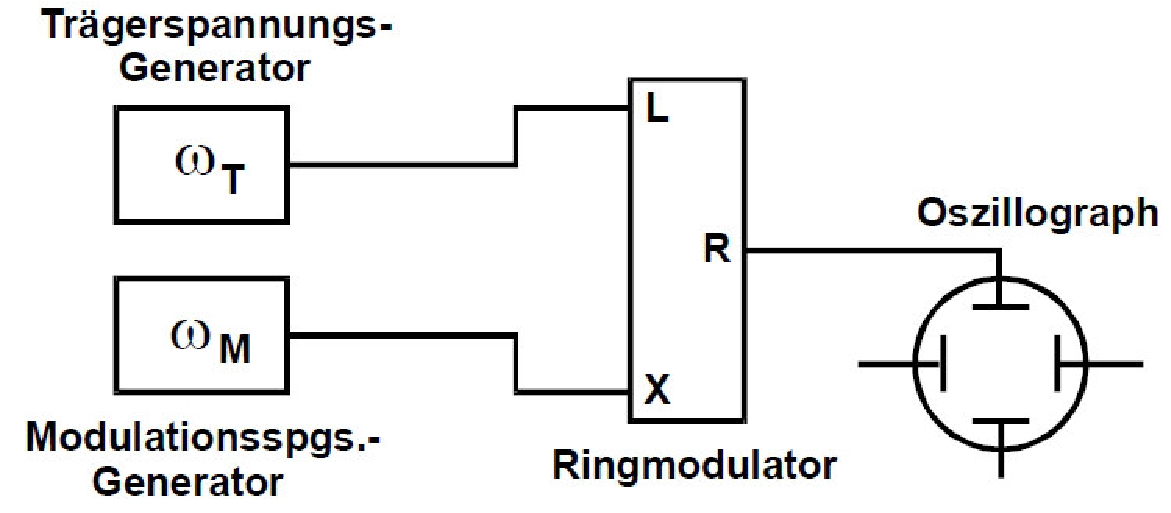
\includegraphics[width = 0.75\textwidth]{../Grafiken/Versuchsaufbau_a.pdf}
	\caption{Die Schaltung mit der die Schwingung einer Amplituden modellierten Spannung aufgenommen wird.\cite{V59}\label{fig:Aufbau_a}}
\end{figure}
Um den Zeitlichen Spannungsverlauf einer amplitudenmodulierten Spannung aufzunehmen wird die Schaltung nach \cref{fig:Aufbau_a} verwendet.
Dabei wird mithilfe eines Oszilloskop die zeitliche Änderung einer durch einen Ringmodulator erzeugten modulierten Spannung aufgenommen.
Das Frequenzspektrum wird aufgenommen, in dem in \cref{fig:Aufbau_a} das Oszilloskop durch ein Frequenzanalyser ersetzt wird.
\newpage
\subsection{Demodulation einer Amplitudenmodulierten Spannung}
\begin{figure}[h!]
	\centering
	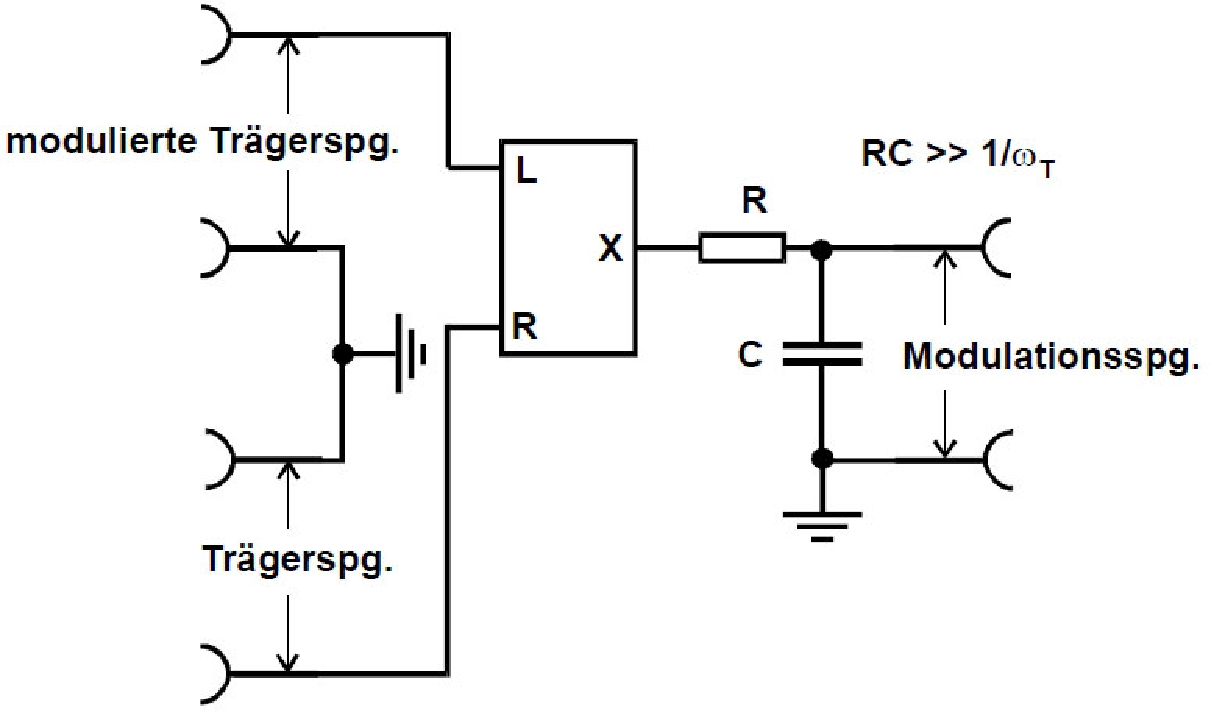
\includegraphics[width = 0.75\textwidth]{../Grafiken/Versuchsaufbau_DemAmplitude_Ringmodulator.pdf}
	\caption{Schaltung für die Demudulation einer Amplitudenmodulierten Spannung.\cite{V59}}
\end{figure}
Die Spannung wird moduliert wie zuvor, mit einem Ringmodulator. 
Dabei wird an die modulierte Trägerspannung an den Eingang L eines Ringmodulators angeschlossen und an Eingang R die unmodulierte Trägerspannung angeschlossen.
An den Ausgang wird ein Tiefpass angeschlossen an dem ein Oszilloskop angeschlossen ist.
Auf dem Zweiten Kanal wird die Modulationsspannung aufgenommen.

\subsection{Modulation mithilfe einer Diode}
\begin{figure}
	\centering
	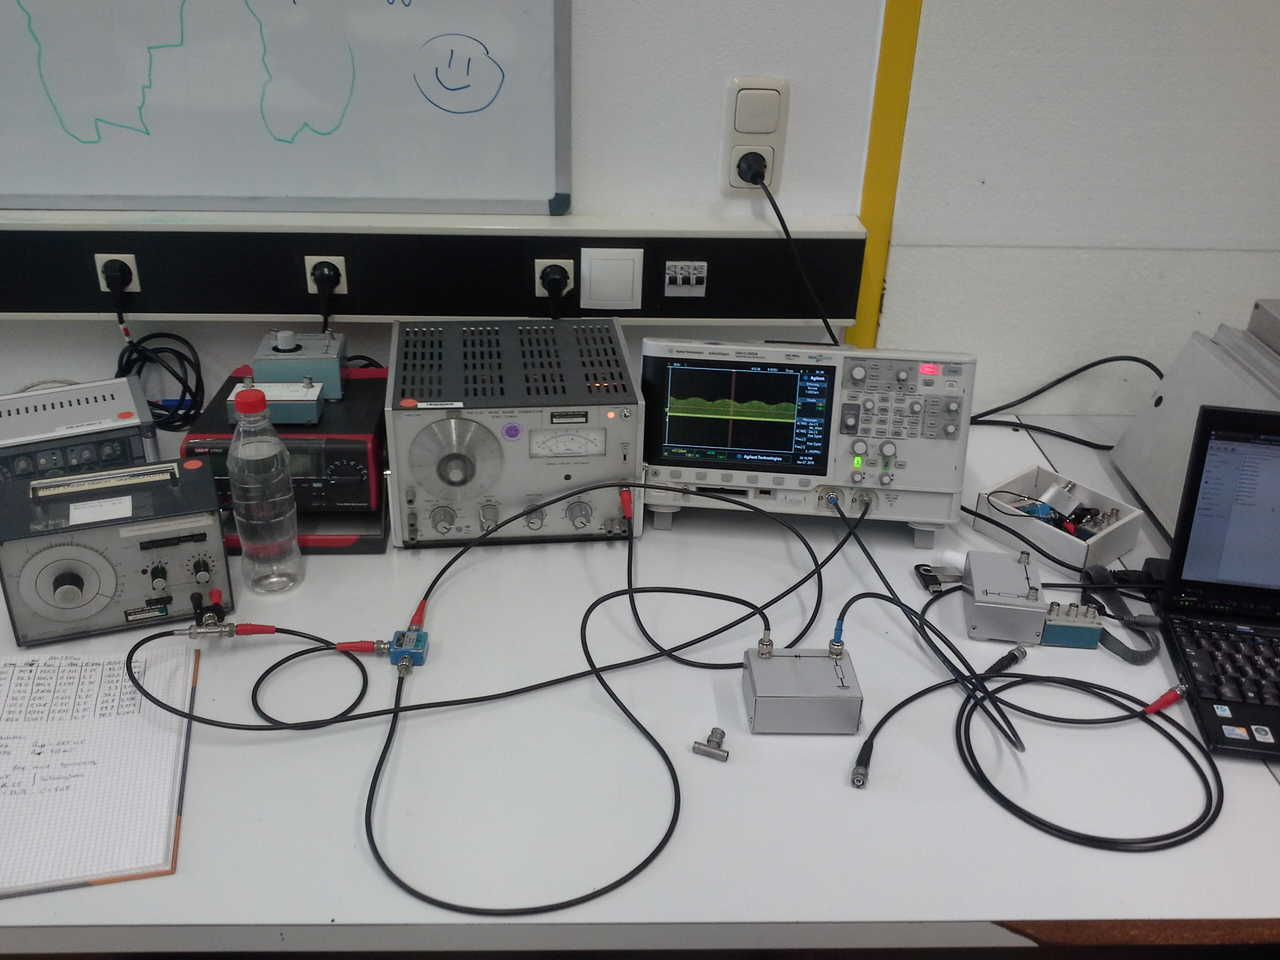
\includegraphics[width = \textwidth]{../Grafiken/Versuchsaufbau_c_AmpModuliertTraeger.jpg}
\end{figure}
Eine Amplitudenmodulation mit Trägerabstrahlung wird erzeugt, mithilfe einer Diode.